% Chapter Template

\chapter{Results} % Main chapter title

\label{Results} % Change X to a consecutive number; for referencing this chapter elsewhere, use \ref{ChapterX}

%----------------------------------------------------------------------------------------
%	SECTION 1
%----------------------------------------------------------------------------------------

\section{Model comparison}

The number of 'gunshots' found by each variant of the model is highlighted in Figure ~\ref{fig:model_comparison}. As the only way to validate the authenticity of these 'gunshots' is through manual checking, there was only time to validate the model that was trained on \cite{Hill2018}'s data from Belize. After validation, 252 'gunshtos' were confirmed to be authentic, meaning 6,912 'gunshots' were deemed to be false positives and giving a model accuracy of 3.65\%. Although the other models haven't been manually validated, it seems a logical assumption, particularly for the Osa Peninsula and Combined models, that the vast majority of 'gunshots' are false positives. For example, if the 'gunshots' returned by the Combined model were all authentic, this would imply that a gunshot was being fired in that area approximately every 16 seconds (24\% of clips) which seems highly unlikely, especially as 1.53\% of audio clips have been manually checked and of these, only 0.08\% contain a confirmed gunshot. Therefore, working on the assumption that the majority of 'gunshots' are false positives, The False Positives and Belize models are the best as they returned the lowest number of 'gunshots'.


\section{Spatio-temporal analysis}

Taking the authenticated gunshots from the Belize model, further analysis was undertaken to explore the temporal patterns of hunting (Figure ~\ref{fig:weekday_plot}). A chi-square test of goodness-of-fit was performed to determine whether gun frequency was independent of the day of the week. Gunshot frequency was equally distributed across the weekdays, $X^2$ (25, $N$ = 252) = 42, $p$ = 0.227.\\

\noindent Further analysis was carried out on the time of day gunshots occured in (Figure ~\ref{fig:timeday_plot}). Gunshots were assigned to either 'morning', 'afternoon' or 'night', mirroring the three periods of the day the audio sensors were set to record. A chi-square test of goodness-of-fit was performed to determine whether gun frequency was independent of time of day. Gunshot frequency was equally distributed across the three periods of the day, $X^2$ (4, $N$ = 252) = 6, $p$ = 0.199. \\

\noindent Gunshot frequency between the six study areas was also compared (Figure ~\ref{fig:area_plot}). A chi-square test of goodness-of-fit was performed to determine whether gun frequency was independent of Area. Gunshot frequency was equally distributed across the six area, $X^2$ (25, $N$ = 252) = 30, $p$ = 0.224.

\begin{figure}
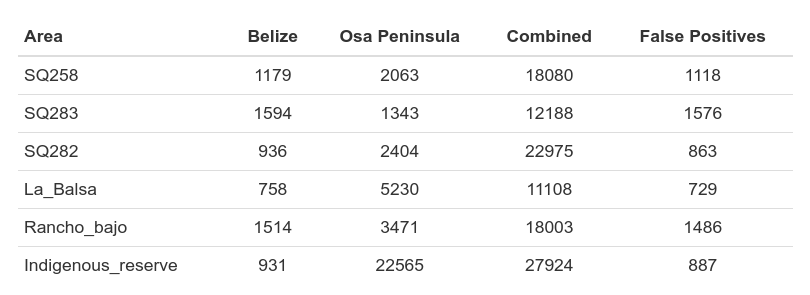
\includegraphics[width=1.2\textwidth,center]{Figures/model_comparison}\caption[Model comparison]{Number of returned 'gunshots' from each version of the convoluted neural network (CNN). The 'Belize' model was trained only on data provided by \cite{Hill2018}, 'Osa Peninsula' was trained on data collected by Jenna Lawson \citep{Lawson2019}, 'Combined' was trained on a combination of the previous two datasets, and 'False Positives' was trained on Jenna's data but all negatives provided were previously identified false positives.}\label{fig:model_comparison}
\end{figure}

\begin{figure}
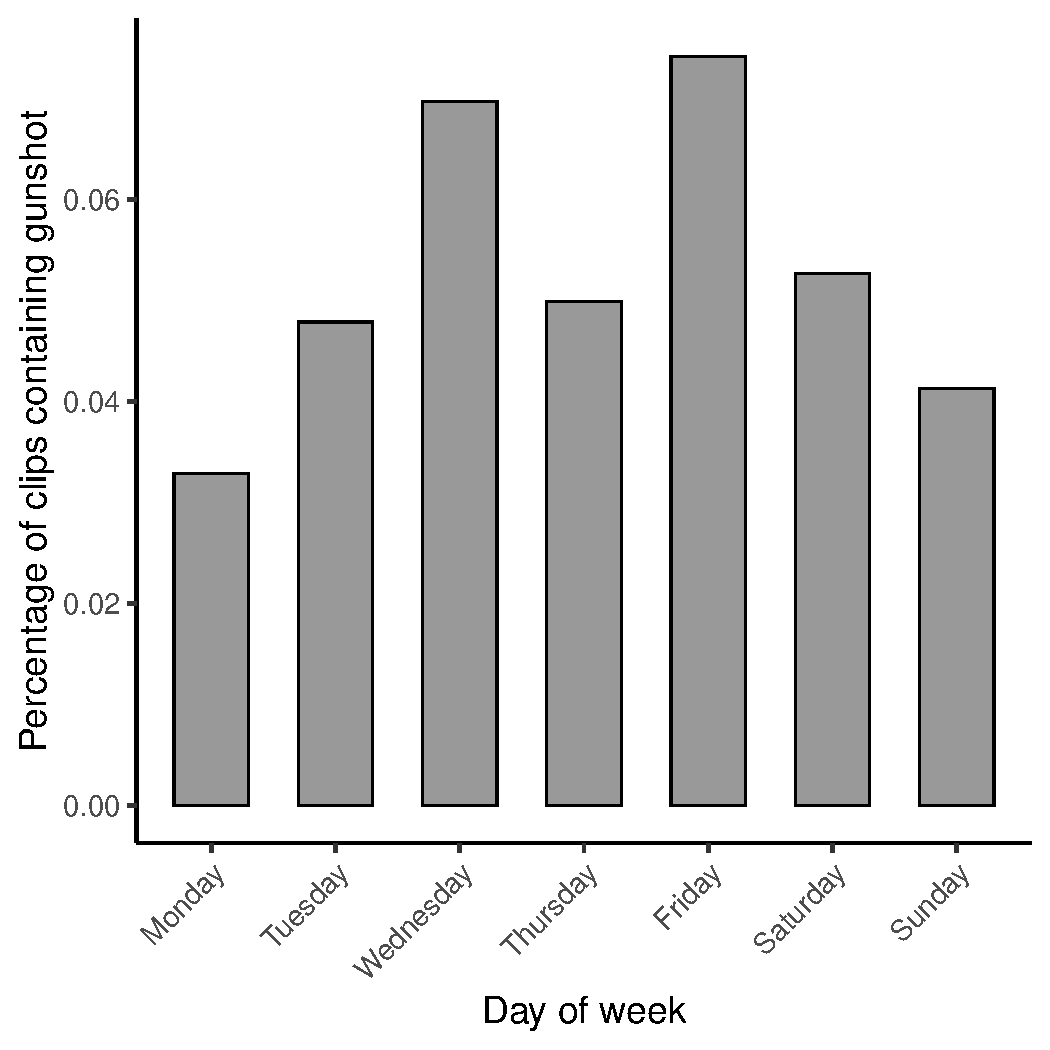
\includegraphics[width=1.2\textwidth,center]{Figures/weekday_plot}\caption[Gunshot frequency by day of week barplot]{Percentage of clips containing a gunshot on each day of the week.}\label{fig:weekday_plot}
\end{figure}

\begin{figure}
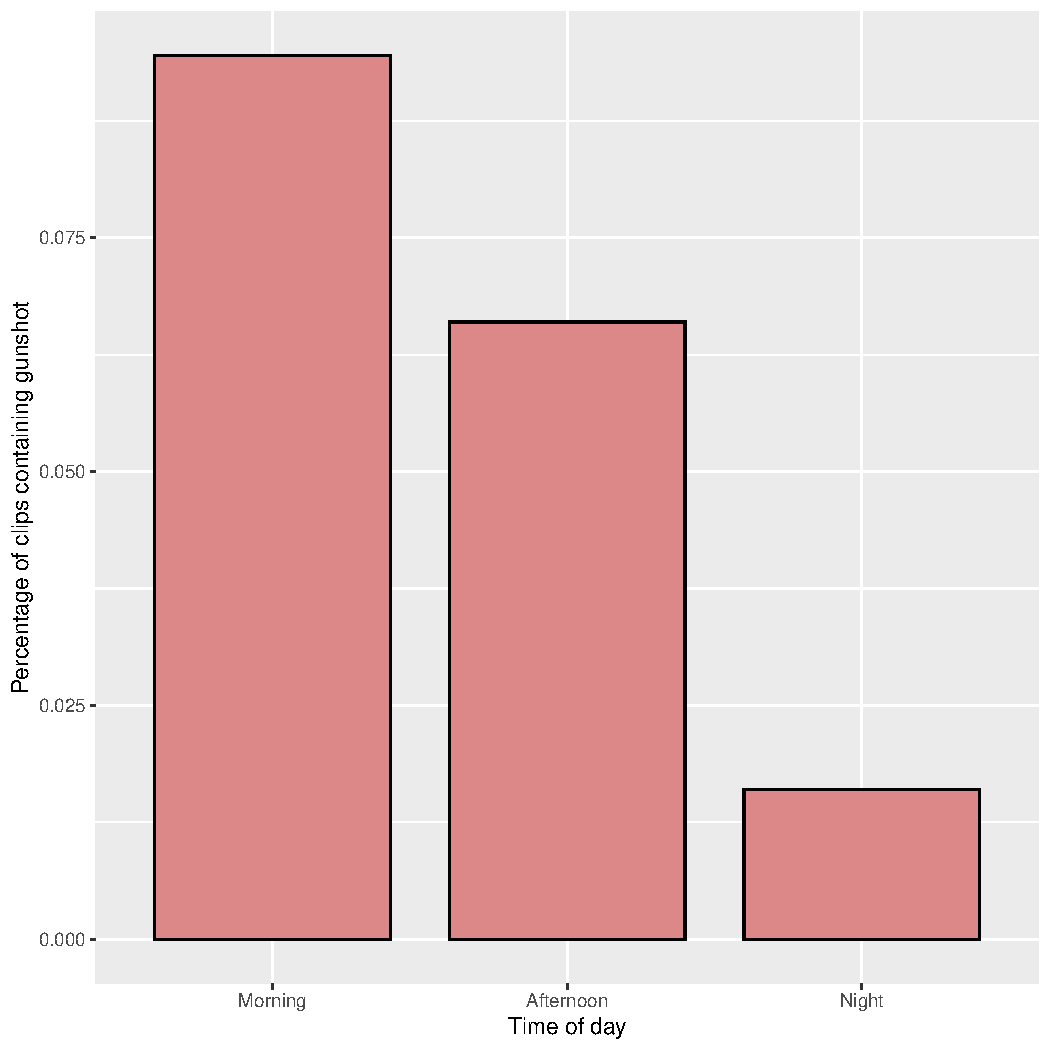
\includegraphics[width=1.2\textwidth,center]{Figures/timeday_plot}\caption[Gunshot frequency by time of day]{Percentage of clips containing a gunshot in each period of the day. 'Morning' was 0500-0930, 'Afternoon' was 1400-1830, and 'Night' was 2100-0300.}\label{fig:timeday_plot}
\end{figure}


\begin{figure}
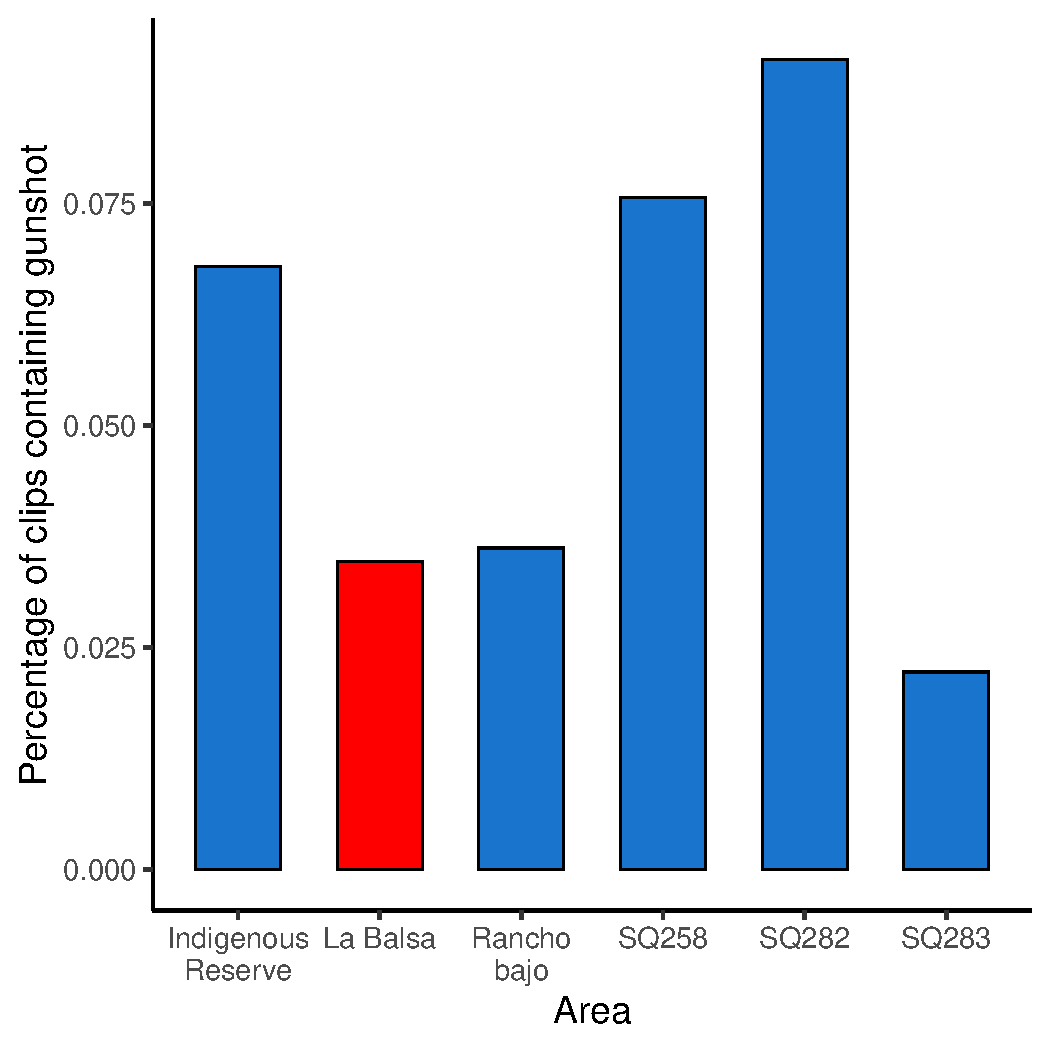
\includegraphics[width=1.2\textwidth,center]{Figures/area_plot}\caption[Gunshot frequency by area]{Percentage of clips containing a gunshot within each of the six regions within the study site.}\label{fig:area_plot}
\end{figure}
